\documentclass{article}
\usepackage[pdftex]{graphicx}
\begin{document}
\title{Root isolation for one-variable polynomials}
\author{Yves Bertot, Assia Mahboubi, Fr\'ed\'erique Guilhot}

\maketitle

\section{introduction}
We want to describe an algorithm that isolates the roots of any
one-variable polynomial with rational coefficients.  This algorithms
constructs a finite list of intervals such that each interval contains
exactly one root of the polynomial and each root is in one of the
intervals.  Such an algorithm can be used as a basic bloc for other
algorithms, for instance to define algebraic numbers or as a component
of cylindrical algebraic decomposition, an algorithm known to decide
systems of inequations between polynomial formulas.

An operation that we will not cover in this paper is an operation
 to reduce the multiplicity of roots: this operation finds a new
polynomial that has the same roots, but where each root is simple.
This can easily be done by computing the greatest
common divisor between the polynomial and its derivative.  In the
following, we thus assume that our polynomial only has simple roots.

The approach we study is based on Bernstein coefficients.  These
coefficients give a discrete approximation of the behavior of a
polynomial in a given closed interval.  We rely on a sufficient
condition concerning these coefficients (let's call this condition
C1): if the Bernstein coefficients, taken in order, have only one
sign change, then the polynomial is guaranteed to have exactly one
root in the corresponding interval.

A first part of our work is to provide a mechanical proof of condition C1.

There is a known transformation of polynomials, so that the roots of a
given polynomial \(P\) inside an interval \((l,r)\) are in one-to-one
correspondance with the roots of a transformed polynomial \(P_1\)
inside the interval \((0,1)\).  Moreover, there is a transformation so
that the roots of \(P_1\) inside \((0,1)\) are in direct
correspondance with the roots of \(P_2\) inside \((0,+\infty)\).
Thus, a sufficient criterion for the existence of exactly one root
between 0 and \(+\infty\) yields a sufficient criterion for the
existence of exactly one root in a bounded interval \((l,r)\).  This is
the essence of a proof of condition C1.  The Bernstein coefficients of
the polynomial \(P\) for the interval \((l,r)\) are the coefficients
of the polynomial \(P_2\).

Descartes' law of signs provides a sufficient criterion for the
existence of exactly one root between 0 and \(+\infty\).  This law
expresses a relation between the number of roots of a polynomial
between 0 and \(+\infty\) and the number of sign changes in the
coefficients of this polynomial.  The number of sign changes is larger
than the number of roots and the difference between the two numbers is
a multiple of 2.  Thus, if the number of sign changes is 1, there is
exactly one root between 0 and \(+\infty\).

For our development, we only prove the simple special case of
Descartes' law of signs for the case where there is only one sign
change.  Expressing Descartes' law on the coefficients of polynomial
\(P_2\) yields directly a law expressed in terms of sign changes for
Bernstein's coefficients of \(P\) with respect to the interval
\((l,r)\).

Another part of our work is to describe dichotomy.  Knowing Bernstein
coefficients for a polynomial and a given interval, it is easy to
compute the Bernstein coefficients for the two half intervals, using
the algorithm known as "de Casteljau".  This increases the precision
at which the polynomials behavior is described, so that condition C1
is guaranteed to eventually hold in the dichotomy process.

Most of our proofs were made using only rational numbers as numeric
values.  Thus, we work with type of numbers where equality and
comparison are decidable and the process we described can effectively
be used in a decision procedure.

When considering only rational numbers, the existence of roots takes a
different meaning: if a polynomial has a single simple real root in an
interval, this root may not be rational.  However, we can use a
corresponding property on rational numbers: there exists a
sub-interval inside which the absolute value of the slope is bounded
below, and such that the values of the polynomial at the sub-interval
bounds have opposite signs.  In a similar vein, the intermediate value
theorem does not hold with rational numbers, but a corresponding
statement, expressed as a bounded-value property, does.  Our proof
development relies on this approach.

This result can then be used for several purposes.  First it opens the
door for a representation of algebraic numbers as equivalence classes
between pairs consisting of a polynomial with rational coefficients
and an interval.  Root isolation makes it possible to decide when two
such pairs describe the same algebraic number.  Second, it can be used
as a basic bloc for a decision procedure deciding logical formulas
with universal and existential quantification where atomic formulas
are comparisons between polynomial formulas.

Berstein polynomials and de Casteljau's algorithm are intensively used
in computer aided design.

\section{Describing roots of a polynomial in the rational setting}
Plan pour cette section
\begin{enumerate}
\item Roots of rational polynomials not necessarily polynomial
\item replace root as a number by a condition on evolution: decompose interval into three part: first part where the polynomial is proved to be strictly negative, second part where the polynomial goes from negative to positive with a slope that is strictly positive, third part where the polynomial is stricly positive
\item In case of Descartes law, impose the slope to be bounded below for all intervals but the first one
\item Using a new form of middle-value theorem: expressed only with rational numbers, applicable only for polynomials
\end{enumerate}

\subsection{Criteria for the existence of a unique root}
When describing the roots of polynomials in a rational setting, we are
faced with the problem that roots I'm not necessarily rational. The
existence of roots is only guaranteed when working with algebraic
numbers or real numbers. To circumvent this difficulty, we only
guarantee a criterion that is strong enough to build a Cauchy sequence
whose limit in the real numbers would be the root. Our criterion is
based on slopes. Indeed, we need to work with cases where the root is
unique. Ensuring that the slope is positive and bounded below or
negative and bounded above helps making sure that there are no two
roots in the area being considered. In the case of positive slopes, we
write the slope requirement for a polynomial \(p\) inside a given interval
\(I\) as follows:
\[exists k, 0 < k \wedge \forall x y, x \in I \wedge y \in I
\wedge x < y \Rightarrow k(y - x) < p(y) - p (x) \]

Depending on the kind of interval that we will consider, we will have
two different ways to express the existence of a single root in the
interval.

\begin{enumerate}
\item If the interval is bounded, we express that the interval can be
  decomposed into three parts, the first part where the polynomial's
  value is always negative (\(I_1\) in Figure~\ref{bounded_decompose}, the second part where the polynomial's
  value goes from negative to positive with a requirement on the
  slope (\(I_2\) in Figure~\ref{bounded_decompose}, and the third part where the polynomial's value is always
  positive (\(I_3\) in Figure \ref{bounded_decompose}).
\begin{figure}\label{bounded_decompose}
\begin{center}

\includegraphics[clip=true,trim= 2cm 7cm 0cm 9cm,scale=0.3]{bounded_decompose.pdf}
\end{center}
\caption{A sufficient criterion for the existence of a single root in a bounded interval}
\end{figure}
\item If the interval is unbounded, we express that the interval can
  be decomposed into two parts, the first part where the polynomials
  value is always negative (\(I_1\) in
  Figure~\ref{unbounded_decompose}, and the second part where there is
  a requirement on the slope with a positive slope (\(I_2\) in
  Figure~\ref{unbounded_decompose}).
\begin{figure}\label{unbounded_decompose}
\begin{center}

\includegraphics[clip=true,trim=2cm 3cm 2cm 9cm, scale=0.3]{unbounded_decompose.pdf}
\end{center}
\caption{A sufficient criterion for the existence of a single root in an unbounded interval}
\end{figure}
\end{enumerate}
\subsection{Bounding the polynomial's value}
While we can't be sure to produce a rational value on which the
polynomial of interest returns the zero value, we at least need to be
able to produce an input for which the polynomial's value is
arbitrarily small. In classical mathematics once we know that the
polynomial takes values of opposite sign at the bounds of an interval,
we know that there is a root for this polynomial in this interval,
thanks to the intermediate value theorem. For this work, we establish
a simplified constructive replacement of the intermediate value
theorem especially for polynomials.

We don't formalize the notion of continuity, but we again rely on
reasoning about slopes. First, we establish that the slope of any
polynomial is bounded in absolute value on any bounded interval. This
gives us a way to establish a property that is stronger than uniform
continuity for polynomials. Starting from an interval and a polynomial
we can produce a coefficient \(k\) so that the variation of the
polynomial between two points \(x\) and \(y\) is smaller than
\(|k\times(y-x)|\) the difference.

Given an arbitrary small and positive \(\varepsilon\), a polynomial
\(p\), and a bounded interval \((l,b)\) so that \(p(l) < 0 < p(r)\),
we want to produce an input \(x_0\) so that \(0 < p(x_0) <
\varepsilon\).  We proceed by taking an upper bound \(k\) of the slope for
this interval and this polynomial and choosing a large number \(n\) so
that \(\frac{r-l}{n} < \frac{\varepsilon}{k}\).  We then consider the
\(n+1\) values \(a_i =l + \frac{i\times (r-l)}{n}\). We then solve a
discrete problem over the values \(a_i\). We simply need to find the
smallest \(a_j\) of these inputs for which the polynomial's value is
positive. The preceding value \(a_{j-1}\) necessarily is a value where
the polynomial is nonpositive. Thanks to the bound on the slope and
because the distance between consecutive \(a_i\)'s is smaller than
\(\frac{\varepsilon}{k}\), we are guaranteed that the value in \(a_i\)
is positive and smaller than \(\varepsilon\).  Note that this approach
makes it possible to bound the polynomial's value in the interval
\((a_{j-1},a_j)\) and to guarantee the existence of a root inside this
interval, however it does not provide for the uniqueness of the root.

Our algorithm is illustrated in figure~\ref{ivt}, where the distance
between the \(a_i\)'s is chosen according to the maximal slope
occurring between \(l=a_0\) and \(r=a_{12}\). The point selected by
our algorithm is \(a_6\), even though there are more roots in the
vicinity of \(a_1\) and \(a_2\) but neither \(a_1\) nor \(a_2\) is a
point where the polynomial takes a positive value.  The point \(a_{11}\) could
also be eligible, but it is not the smallest one.
\begin{figure}
\label{ivt}
\begin{center}

\includegraphics[clip=true,trim=0cm 9cm 2cm 9cm,scale=0.5]{ivt.pdf}
\end{center}
\caption{Bounding a polynomials value}
\end{figure}

\section{A simple form of Descartes' law of signs}
\subsection{Mathematical proof}
Let's first describe a simple graphical argument based on curves for polynomial functions between 0 and \(+\infty\), as shown in figure~\ref{graph-desc}.
\begin{figure}
\label{graph-desc}
\begin{center}
\includegraphics[width=0.5\textwidth]{alternated2.pdf}
\end{center}
{(a) non-negative coefficients, first one non-zero,\\
(b) non-negative coefficients, first one zero,\\
(c) first coefficient negative, all others non-negative,\\
(d) one sign change, first coefficient zero,\\
(e) one sign change, first coefficient negative}

\caption{Classes of polynomials with or without
sign change}
\end{figure}
To describe our proof, we assume that new polynomials are built from
existing ones by multiplying them by the polynomial \(X\) and adding a
constant; an operation that is known as ``Horner's scheme''.
Polynomials with one sign change and a positive principal coefficient
are obtained by starting with a positive constant, applying Horner's
scheme a certain number of times with non-negative constants, then
applying it a negative constant, and then applying it again a certain
number of times with non-positive constants.

Polynomials with only non-negative coefficients have curves which look
like the curves (3.1-a) or (3.1-b) depending on whether the first
coefficient is 0, adding a positive coefficient to a polynomial of the
form (a) or (b) yields a polynomial of the form (a), multiplying a
polynomial of the form (a) or (b) by the polynomial \(X\) yields a new
polynomial of the form (b).  Thus, Horner's scheme with non-negative
constants keeps polynomials in the (a-b) form.  Then, when applying
Horner's scheme with a negative coefficient (thus introducing a sign
change), the multiplication by \(X\) first builds a polynomial of the
(b) form, and adding a negative constant, one obtains a curve whose
shape is given by (c).  From then one, multiplying a polynomial of the
form (c), (d), or (e) by \(X\) yields a a polynomial of the (d) form; adding a
negative constant to a polynomial of the form (d) or (e) yields a
polynomial of the (e) form.  Polynomials of the form (d) or (e)
share the following characteristic: there exists a positive value
\(x\), so that the polynomial has a negative value between 0 and
\(x\), and the slope of the curve is strictly positive above
\(x\).  Because of the slope condition, we can also find a point where
the polynomial is positive.

Let us now give a more precise proof, outlining the concepts that are
used in the formal proof.

{\sf A lemma on slopes of products of functions: If two positive functions \(f\)
and \(g\) have slopes larger than \(k_f > 0\) and \(k_g > 0\) on the interval
\([a,b]\), then the slope
of the product \(fg\) is larger than \(k_fg(a) + f(a)k_g\).  }

We first define an invariant that is used for polynomials with only
positive coefficients.  The important characteristics are the
following ones (grouped in our development under the name {\tt inv2}):
there exists a positive \(x\) such that \(x * P(x)\)
can be made arbirarily close to 0, the value of \(P(x)\) is positive,
the value of \(P\) in \([0,x]\) is below \(P(x)\), and the polynomial
is increasing above \(x\).  We then show that if any polynomial \(P\)
satisfies these important characteristics, and \(a\) is a non negative
number, then the polynomial \(a + X * P\) also satisfies them.

This is the step case in a proof by induction concerning polynomials
with all non-negative coefficients and at least one positive coefficient.

We can then address polynomials with exactly one sign change.  We want to
show that these polynomials have exactly one root.  We exhibit the three
intervals described in the previous section by giving two values \(x_1\) and \(x_2\) and \(k\) such that the polynomial is negative for every positive \(y\) smaller than \(x_1\), the polynomial is positive in \(x_2\), and the slope between
any two values above \(x_1\) is positive.
\begin{enumerate}
\item Consider a polynomial \(P = a_0 + a_1 x + a_n x^n\)
of degree \(n\), with two natural numbers \(i\), \(j\) such that
\(i < j\), \(a_i < 0\), \(0 < a_j\), and
\[\forall l, l < j \Rightarrow a_k \leq 0\]
\[\forall l, j \leq l \Rightarrow 0 \leq a_l\]
\item Prove that there is exactly one root between 0 and \(+\infty\)
\item Expressed in the following form: there exists \(x > 0\), \(k > 0\),
\(\forall y, 0 < y \leq x \Rightarrow P(y) < 0\) and
\(\forall y z, x \leq y < z \Rightarrow k (z - x) < P(z)-P(x) \).
\item The proof is done by two inductions:
\item First prove that every polynomial with only strictly positive coefficients
is strictly positive and increasing in \((0,+\infty)\)
\item Then prove by induction on \(j\)
\item Consider the truncated polynomial
\(P_t = a_1 + a_2 x + a_j x^{j-1} + a_n x^{n-1}\): we know that \(a_0 \leq 0\)
and there are two cases:
\begin{enumerate}
\item If \(P_t\) has no alternance, then \(a_0 < 0\) and the previous lemma
is satified for \(a_1 x + a_n x ^ n\) , this makes it possible to find
an \(x_1\) such that \(x_1 \times P(x_1) < - a_0\).  Thanks to the lemma
on slopes, the slope of the polynomial \(X \times P\) above \(x_1\) is larger
than \(P_t (x)\), this is enough to find a value \(x_2\) such that
\(P(x_2)\) is positive.
\item If \(P_t\) has one alternance, then the induction hypothesis provides
a relevant \(x_{1t}\) and \(k_t\) for this polynomial.  We can consider the
value \(y = x_{1t} - a_0/{k_tx_{1t}}\).  This value is larger than \(x_{1t}\).
Thanks to the properties of \(k_t\) we know
that\(y * P_t(y) > k_t (y - x_{1t}) > - a0\) and thus, \(P(y) > 0\)
\item Using the middle-value theorem, we exhibit two new values \(z\) and \(x\),
 such that \(x_{1t} < z < x < y\), \(- k_t x_{1t} < P_t(z) < 0 < P_t(x) < a_0/y\)
\item Obviously, \(P\) is negative below \(x_{1t}\),
\item Thanks to the lemma at the beginning of this section,
\(X * P_t\) has a slope larger than \(k * x_{1t} + P_t(z) > 0\) between
\(z\) and \(x\), so that \(P\) is negative in this interval,
\item Because \(P_t\) is increasing between \(x_{1t}\) and \(z\), \(P_t\) is
negative in
\item Because \(P_t\) is increasing between \(x_{1t}\) and \(x\), we can show
that \(P\) is negative between \(x_{1t}\) and \(x\)
\item  Thanks to the lemma at the beginning of this section,
the slope of \(P\) above \(x\) is larger than
\(k = P_t(x) + k_t x\).
\end{enumerate}
\end{enumerate}
\subsection{Formal description}
\begin{enumerate}
\item The functions that describe
\end{enumerate}
\section{From Bernstein to Descartes}

In this section, we clarify the polynomial transformations that link
the problem of finding the roots of a polynomial inside an arbitrary
bounded interval \((l,r)\) successively with the problem of finding
the roots of an other polynomial inside the interval \((0,1)\) and
with the problem of finding the roots of yet another polynomial inside
the interval \((0,+\infty)\).

\subsection{A criterion for the interval \((1,+\infty)\)}
The law of signs gives us a sufficient condition to determine when the
unbounded interval \((0,+\infty)\) contains exactly one root for a
polynomial. Through a change of variable, we obtain a similar
criterion for the interval \((1, +\infty)\).

 The polynomial \(P(x)\)
has exactly one root in the interval \((1,+\infty)\) if and only if
the polynomial function \(y \mapsto P(y+1)\) has exactly one root in
the interval \((0,+\infty)\). Expressed in termes of the
coefficients \(a_i\) of the polynomial
\(P\), we have \[P(y+1)= \sum_{i=0}^{n} a_i (y+1)^i = \sum_{k=0}^{n}
\sum_{i=k}^{n}a_i\left(\begin{array}{c}i\\k\end{array}\right) y^k\]

Thus, if we apply Descartes's law of sign on the coefficients
\(\sum_{i=k}^{n}a_i\left(\begin{array}{c}i\\k\end{array}\right)\), we
can obtain a sufficient criterion for the existence of exactly one
root of polynomial \(P=\sum_{i=0}^{n}a_ix^i\) in the interval
\((1,+\infty)\).

With our approach to describe unique roots of polynomials inside
unbounded intervals, we can easily establish a correspondence between
the way we express existence for the two intervals.
\subsection{A criterion for the interval \((0,1)\)}
Descartes' law of signs works for unbounded intervals.  In this
section, we see how to cover also bounded intervals.

Then, there is a trick to transfer the criterion's explicit power on a
bounded interval, the interval between zero and one. This trick relies
on reversing the polynomial's list of coefficients.  Obviously, the
number of sign changes in a list of coefficients is the same as the
number of sign changes in the reversed list.

However, the roots of a polynomial on the interval \((1,+\infty)\)
infinity are in one-to-one correspondence with the roots of the
reversed polynomial between zero and one. This is due to the following
equation:
\[\sum_{i=0}^{n}a_i x^i = x^n\times\sum_{i=0}^{n}x^{i-n}\]
We can now perform another change of variable, here \(y=1/x\) and a
change of index \(j=n-i\) in the sum.
\[\sum_{i=0}^{n}a_i x^l = (\frac{1}{y})^n \sum_{j=0}^{n}a_{n-j} y^j\]
The polynomial \(\sum_{j=0}^{n} a_{n-j}y^j\) is exactly the reversed
polynomial, and the expression \((\frac{1}{y})^n\) never becomes 0 for
\(y\in (0,1)\).  Thus, \(x\) is a root of the polynomial between \(1\)
and \(+\infty\) if and only if \(y=x^-1\) is a root of the reversed
polynomial between \(0\) and \(1\).

For instance, we can consider the polynomial \(P(x) = x^3 - 5/2 x^2 - 2 x + 3/2\),
the reversed polynomial is \(Q(x) = 3/2 x^3 - 2 x^2 - 5/2 x + 1\) and after 
the variable change we obtain the polynomial \(3/2 x^3 + 5/2 x^2 - 2 x - 2\)
which exhibits only one sign change.  This predicts that the polynomial has
exactly one root between 0 and 1, and indeed the three roots of the initial
polynomial are -1, 1/2, and 3.  This is illustrated in
figure~\ref{invert} where the curve with a solid line is the curve for the
polynomial \(P\), while the curve with a dashed line is the curve for
the polynomial \(Q\), which has a single root between 1 and \(+\infty\).
\begin{figure}\label{invert}
\begin{center}
\includegraphics[clip=true,trim=3cm 5cm 3cm 14cm, width=0.5\textwidth]{invert.pdf}
\end{center}
\caption{Curves of \(x^3 -\frac{5}{2} x^2 - 2 x +
  \frac{3}{2}\)
and its reverse \(\frac{3}{2}x^3 -2 x^2 - \frac{5}{2} x + 1\)}
\end{figure}

With our approach to describe unique roots of polynomials, we need to
establish a correspondence between the current time for unbounded
intervals and the criterion for bounded intervals. As this proof also
involves composition with the inverse function, this is one of the
trickiest proofs in our developments, in particular when we need to
find the sub-interval and the slope that is guaranteed on this
interval.  This is a place where our constructive intermediate value
theorem plays a role.

\subsection{handling arbitrary bounded intervals}

The next step is to relate the roots of any polynomial inside an
arbitrary interval\footnote{We name the bound \(l\) for {\em left} and
  \(r\) for {\em right}.} \((l,r)\) with the roots of another
polynomial inside the interval \((0,1)\).  This is done with another
change of variable, this time \(x= (r-l) y + l\); in other words, the
polynomial function which maps any \(x\) to \(p(x)\) has a root
between \(l\) and \(r\) if and only if the polynomial function which
maps any \(y\) to \(p((r - l) y + l)\) has a root between 0 and 1.

This is illustrated in figure~\ref{expand-translate}, where the shape
of the curve for the polynomial \(\frac{x^3}{8} - \frac{x^2}{8} + 3
x\) inside the interval \((2,4)\) is reproduced by the shape of the
curve for the polynomial \(x^3 -\frac{5}{2}x^2-2x+\frac{3}{2}\) inside
the theorem \((0,1)\).
\begin{figure}
\begin{center}\label{expand-translate}

\includegraphics[clip=true,trim=4.5cm 18cm 2cm 3cm, width=0.5\textwidth]{expand-translate.pdf}
\end{center}
\caption{Curves of a polynomial inside \((2,4)\) and the
  corresponding transformed polynomial between \((0,1)\)}
\end{figure}
\subsection{Recapitulating operations}
In our formal development, we defined three operations for
translating, expanding, and reversing the list of coefficients and we
simply defined the list of Bernstein coefficients as the result of
performing these operations.  We then showed how these operations
behave with respect to the criteria concerning our sufficient criteria
for the existence of exactly one root in intervals.  In particular:

\begin{itemize}
\item translating a polynomial preserves the criterion for existence
of exactly one root in bounded intervals and in unbounded intervals,
\item expanding a polynomial preserves the criterion for existence of
  exactly one root in bounded intervals,
\item reversing the list of coefficients maps a polynomial satisfying
  the criterion for the existence of exactly one root in the unbounded
  interval \((1,+\infty)\) into a polynomial satisfying the criterion
  for the existence of exactly one root in the bounded interval \((0,1)\).
\end{itemize}
\end{document}
%%% Local Variables:
%%% mode: latex
%%% TeX-master: t
%%% End:
